    % ------ CORNELL PHYS 2210 FINAL POSTER ------------------%
 
    %=========================================================%
    %                                                         %
    %    _______       __                                     %
    %  /   ------.   / ._`_                                   %
    % |  /         ~--~    \                                  %
    % | |             __    `.____________________ _^-----^   % 
    % | |  I=|=======/--\=========================| o o o |   % 
    % \ |  I=|=======\__/=========================|_o_o_o_|   %
    %  \|                   /                       ~    ~    %
    %    \       .---.    .                                   %
    %      -----'     ~~''                                    %
    %                                                         %
    %=========================================================%

    % ------ Template by: Madeline Jennings ------------------%








%----------------------------------------------------------------------%
%                        ||| PREAMBLE |||                              %
%----------------------------------------------------------------------%

\documentclass{article}

%\______________________________________________________________________________/%
% -- PACKAGES --%

\usepackage{graphicx} % Required for inserting images
\usepackage[svgnames]{xcolor} % To change the font color
\usepackage{enumitem} % Required for customizing lists

\usepackage[ % Page size and margins
    paperwidth=42in,
    paperheight=38in,
    margin = 1in
]{geometry}

\usepackage{anyfontsize} % To use arbitrary font sizes
\usepackage{tikz} % Necessary for figures
\usepackage{pgfplots} % Often loaded with TikZ environments
\pgfplotsset{compat=1.18} % Set compatibility level
\usepackage{capt-of} % For captions outside of floats
\usepackage{multicol} % For multiple columns
\usepackage{blindtext} % For placeholder text
%\______________________________________________________________________________/%


%\______________________________________________________________________________/%
% -- SET COLUMN PARAMETERS --%

\columnsep=50pt % Set the space between columns
\columnseprule= 2pt % Set the thickness of the line between columns (optional)

% Redefine \section command
\renewcommand{\section}[1]{
    \begin{center}
    \begin{tikzpicture}
        \draw node[fill=red!10,
        text width = 0.9\linewidth,
        text centered,
        inner sep = 30pt,
        rounded corners = 5pt,
        draw = red!80]{\textbf{#1}};
    \end{tikzpicture}
    \end{center}}
%\______________________________________________________________________________/%










%----------------------------------------------------------------------%
%                      ||| START OF DOCUMENT |||                       %
%----------------------------------------------------------------------%

\begin{document}

%\______________________________________________________________________________/%
% -- TITLE SECTION -- %

\begin{center}
    \fontsize{55}{65}\selectfont

    \begin{tikzpicture}
        \draw node[
            fill=red!10,
            text width=0.95\linewidth,
            text centered,
            inner sep=30pt,
            rounded corners=5pt,
            draw=red!80
        ]{
            \makebox[\textwidth]{
                \begin{minipage}{0.80\textwidth}
                    \centering
                    \textbf{Audio Spectrum Analysis of Natural Harmonics on a Vibrating Guitar String}
                    \\[1cm]
                    \fontsize{50}{60}\selectfont
                    Madeline Jennings, Isaac Kahn, Phawat Leechasan
                    \\[0.5cm]
                    Cornell University
                \end{minipage}
                \hfill
                \begin{minipage}{0.2\textwidth}
                    \centering
                    \includegraphics[scale=0.30]{cornell.png} % Cornell Logo
                \end{minipage}
            }
        };
    \end{tikzpicture}
\end{center}

\vspace{2cm} % Vertical space between title section and poster content
%\______________________________________________________________________________/%



%\______________________________________________________________________________/%
% -- POSTER CONTENT -- %

\begin{multicols*}{3} % Start of 3-column layout
    \fontsize{40}{50}\selectfont % 40pt font size with 50pt line spacing

    %------------------------------------------%
    %            ||| ABSTRACT |||              %
    %------------------------------------------%

    \section{Abstract}
    This project investigates the characteristics of natural harmonics on a vibrating guitar string.
    Our goal was to analyze the conditions under which they occur (namely, how the thickness, tension and playing position of the string affect the resultant sound).
    We used a Fast Fourier Transform (\textbf{FFT}) to analyze the harmonics produced on each fret of each string and found that \textbf{[1]} the frets where harmonics occur are the same for each string.
    We further found that \textbf{[2]} harmonics on these frets form the same interval from the open string across all strings, and \textbf{[3]} the presence of a harmonic on a given fret can be predicted by its proximity to \textbf{standing wave} nodes. 
    \\
    
    %------------------------------------------%
    %            ||| INTRODUCTION |||          %
    %------------------------------------------%

    \section{Introduction}

    Guitarists have observed that plucking a string while lightly pressing it above a fret wire causes major changes in the resultant sound. 
    In some cases, the fingering deadens the string, muting it almost entirely, and at other frets, a \textbf{natural harmonic} emerges.
    Natural harmonics have a distinct, bell-like tone, different from the sound produced by normal fretting. To hear an \textcolor{red}{\textbf{example} of a \textit{harmonic} and a \textit{dead string}}, scan the QR code below.

    \begin{minipage}[t]{0.38\linewidth}
    % QR Code with a link to example recordings
    \vspace{0pt}
    \includegraphics[scale=0.30]{QR.png}
    \end{minipage}
    \begin{minipage}[t]{0.58\linewidth}
    \vspace{0pt}
    \hangindent=0pt
    \hangafter=0
    The harmonics on different frets vary greatly in their tonal qualities, and it is not at first obvious to predict which frets will produce strong harmonics or their component frequencies. Some may pro-
    \end{minipage}
    duce a sound an octave higher than from normal fretting, while others produce sounds that differ by another interval.
    \\

    %------------------------------------------%
    %            ||| EXPERIMENT |||            %
    %------------------------------------------%

    \section{Experiment}

    For each fret on each string of the guitar, we attempted the mechanism that produces the natural harmonic. We did this about 10 times for each fret, as sometimes the mechanism is not properly achieved on the first try.
    The resultant sound was recorded on a Shure SM57 microphone and stored in .flac format.
    The area surrounding the microphone was soundproofed to minimize background noise, and the location of the guitar relative to the microphone as well as the plucking position were held constant throughout the experiment.  
    Some supporting measurements were taken, such as the position of each fret (in cm) along the string, and other qualities such as the diameter, material and tension on each string could be found on the container.
    The figure below is of the \textcolor{red}{\textbf{experimental setup}}.

    \begin{minipage}[t]{0.54\linewidth}
    % QR Code with a link to example recordings
    \vspace{0pt}
    \includegraphics[scale=0.30]{setup.jpg}
    \end{minipage}
    \begin{minipage}[t]{0.40\linewidth}
    \vspace{0pt}
    \hangindent=0pt
    \hangafter=0
    After reviewing the audio clips and flagging recordings with audible harmonics, a clearest recording was selected from each, of the 10 or so trials. This is simply the instance with the l-
    \end{minipage}
    \\

    -east background noise and the loudest harmonic.
    A FFT was then performed using NumPy on each recording to determine its constituent frequencies and their respective amplitudes.

    %------------------------------------------%
    %            ||| RESULTS |||               %
    %------------------------------------------%

    \section{Results}

    The most immediate observation, prior to performing any FFT, was that the frets along the string with audible harmonics were the same for each string.
    Though their constituent frequencies differed, the intervals between the harmonics and the frequency of the open string were consistent across strings as well. For example, the most audible ha-
    
    \begin{minipage}[t]{0.45\linewidth}
    % QR Code with a link to example recordings
    \vspace{0pt}
    \begin{tabular}{|c|p{10cm}|}
        \hline
        \textbf{Fret} & \textbf{Interval From Open String} \\ \hline
        4 & M3 \\ \hline
        5 & Octave (x2) \\ \hline
        7 & P5 \\ \hline
        9 & M3 \\ \hline
        12 & Octave \\ \hline
        16 & M3 \\ \hline
        19 & P5 \\ \hline
        \end{tabular}
    \end{minipage}
    \begin{minipage}[t]{0.52\linewidth}
    \vspace{0pt}
    \hangindent=0pt
    \hangafter=0
    -rmonic frequency on the 5th fret of the low E string is roughly 325Hz (E4), which is two octaves above the open string.
    On the 5th fret of the D string, it is roughly 577Hz (closest to D5), which is also two octaves above the open string.
    \end{minipage}
    \\

    A table of the frets with audible \textcolor{red}{harmonics and their \textbf{intervals} from the open string} is shown above. 


    %------------------------------------------%
    %            ||| DISCUSSION |||            %
    %------------------------------------------%

    \section{Discussion}

    The widely accepted hypothesis that frets closer to standing wave nodes will have prominent harmonics is supported by our data. 
    The graph below shows the \textcolor{red}{number of \textbf{nodes} within 0.5$\%$ of the string's \textit{length} to a given \textbf{fret}.}
    The frets with high node counts (19, 12, 7) have clear harmonics with strong frequencies in their FFT plots that stand out from noise.
    It is evident that the \textbf{length} of the string impacts where along the string harmonics will occur, \textit{as opposed to} the tension, mass or thickness, which seem to impact the \textbf{frequencies} of the harmonic instead.
    \\
    \begin{minipage}{\linewidth}
        \centering
        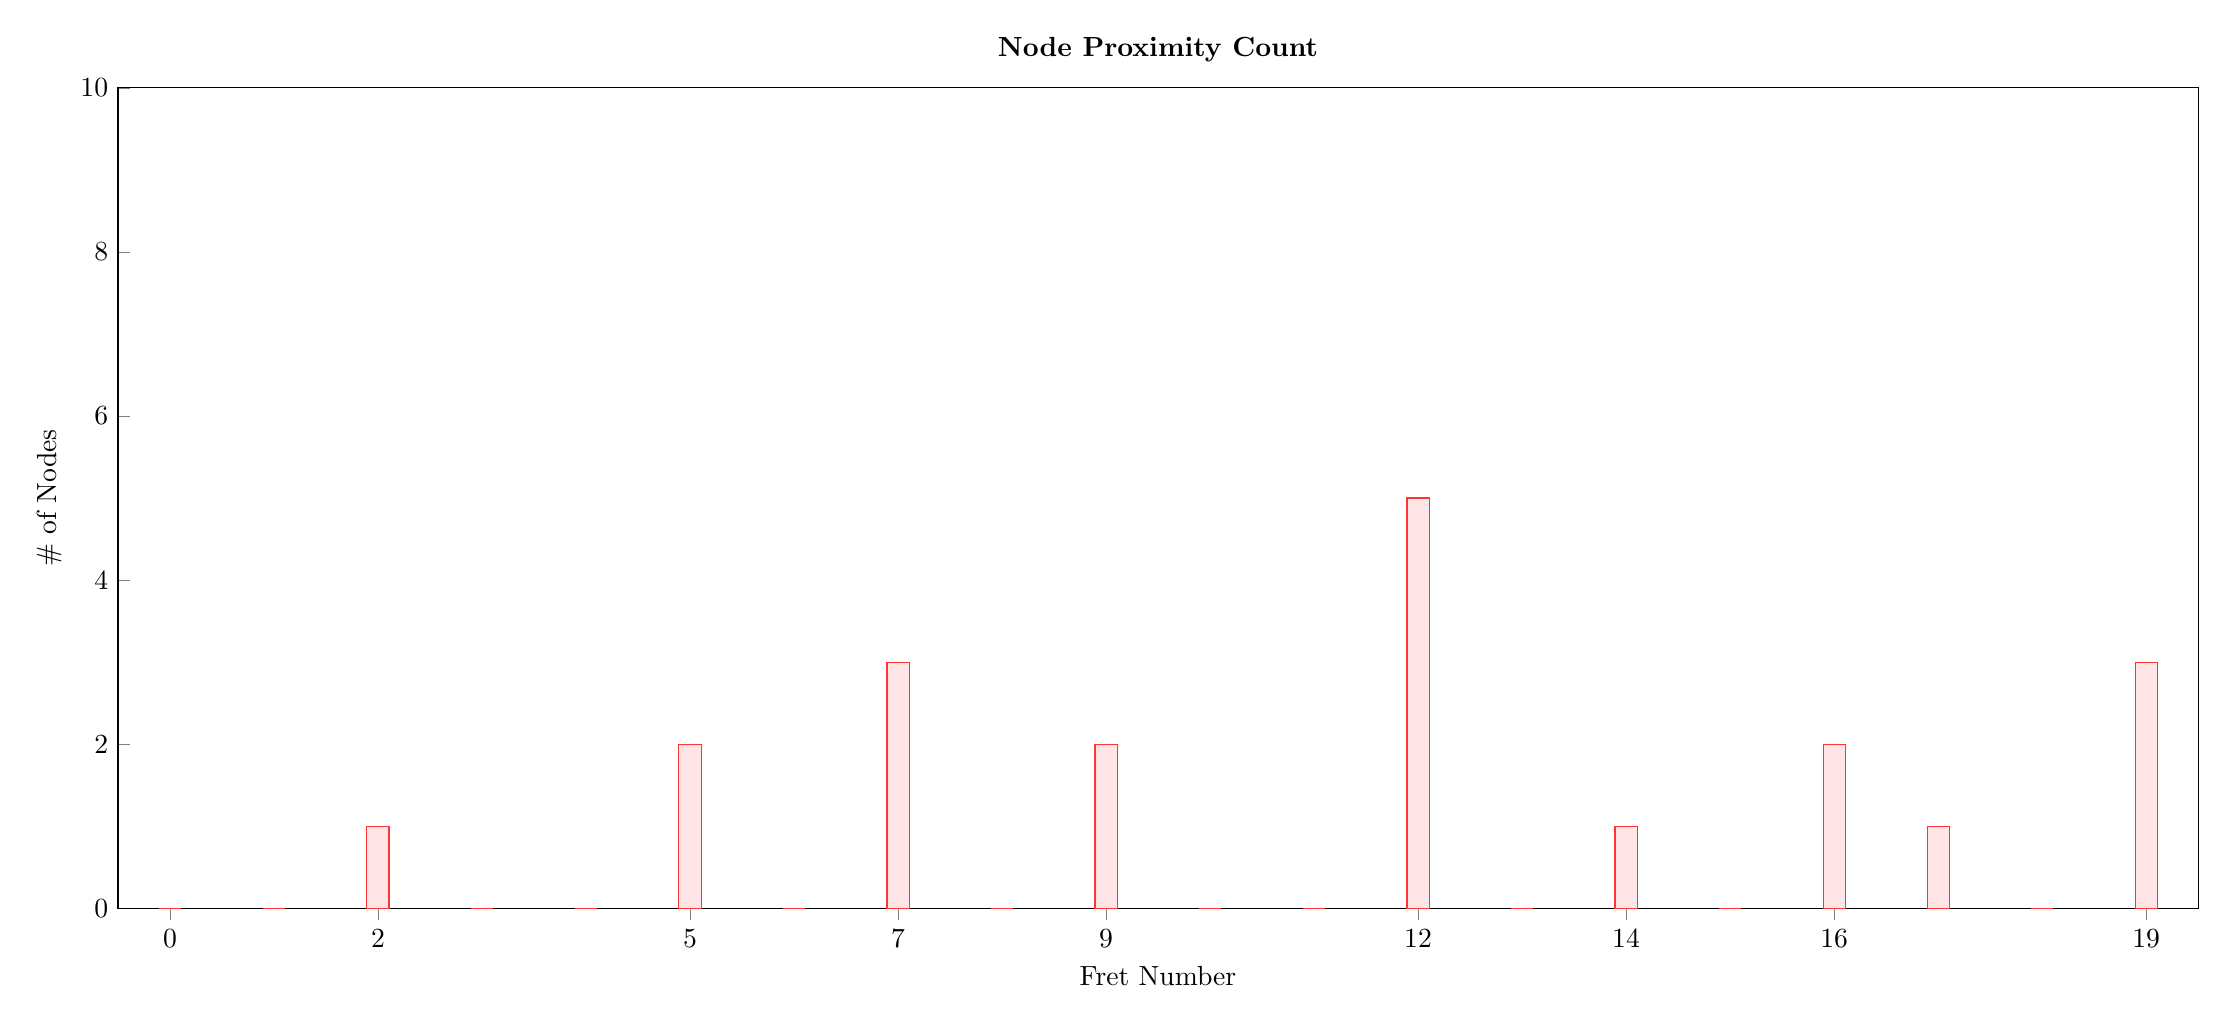
\begin{tikzpicture}

        \begin{axis}[
            title={\textbf{Node Proximity Count}},
            ybar,
            ymin=0, ymax=10,
            xmin=-0.5, xmax=19.5,
            xtick={0,2,5,7,9,12,14,16,19},
            ytick={0,2,4,6,8,10},
            xlabel={Fret Number},
            ylabel={\# of Nodes},
            bar width=8pt,
            width=28cm,
            height=12cm,
            xtick pos=bottom,
            ytick pos=left,
        ]
        \addplot[
            fill=red!10,
            draw=red!80,
            ]
            coordinates {
            (0,0) (1,0) (2,1) (3,0) (4,0)
            (5,2) (6,0) (7,3) (8,0) (9,2)
            (10,0) (11,0) (12,5) (13,0) (14,1)
            (15,0) (16,2) (17,1) (18,0) (19,3)
        };

        \end{axis}
        \end{tikzpicture}
    \end{minipage}



    %------------------------------------------%
    %            ||| CONCLUSION |||            %
    %------------------------------------------%

    \section{Conclusion}

    Our analysis has led to several key conclusions:
    
    \begin{enumerate}[label=\textbf{\arabic*.)}, leftmargin=1.5em]
        \item Natural harmonics occur at the \underline{same frets for each string.}
        \item The \underline{intervals} between a fret's  harmonic and the open string are invariant across strings.
        \item The presence of a fret's harmonic can be predicted reasonably well by the \underline{distance from the fret to a node.}
    \end{enumerate}

    % Areas for future research
    One interesting area of research for future investigators would be to examine the dynamics of \textbf{artificial} harmonics, colloquially known as “pinch” harmonics. These are performed on an electric guitar with a special picking technique, and produce very different results.

    %------------------------------------------%
    %            ||| Additional |||            %
    %------------------------------------------%

    \section{Additional Reading}
    
    More data, measurements, audio recordings, and code used in this project can be found at our GitHub repo:
    \underline{https://github.com/zhav0ronok/phys2210-final}
\end{multicols*}
%\______________________________________________________________________________/%


\end{document}

